%!TEX encoding = UTF-8 Unicode
%!TEX root = ../lect-week13.tex

%%%

\ifkompendium\else

\begin{Slide}{Uppsamling: obligatoriska moment}\SlideFontSmall
\begin{itemize}
\item Kolla vilka oblikatoriska moment du har kvar här:
\url{http://cs.lth.se/pgk/sam}
\item Sök på din födelsemånad/dag, tex 0102 för andra januari.
\item Du måste ha gjort \Emph{kontrollskrivning} och vara godkänd på alla \Emph{laborationer} (utom rekommenderade men valfria w12\_survey) och vara godkänd på \Emph{projektet} för att få tentera \code{pgk}!
\item Din ev. \Emph{samarbetsbonus} (max 5p) från kontrollskrivningen gäller endast första ordinarie tentamenstillfälle.
\item Läs \Alert{alla} instruktioner \Alert{noga} och \Alert{anmäl dig} här: \\
\href{http://www.student.lth.se/studieinformation/anonyma-tentor/}{www.student.lth.se/studieinformation/anonyma-tentor}
\item Du måste vara \Emph{godkänd} på alla obligatoriska labbar och projektet \Alert{innan du får påbörja pfk} \href{http://cs.lth.se/edaa01vt}{EDAA01}
\item Använd återstående \Emph{resurstider} för \Alert{redovisning av labbar/projekt}.
\end{itemize}
\end{Slide}

\begin{Slide}{CEQ -- Course Experience Questionnaire}\SlideFontSmall
\begin{itemize}
\item Görs på hela LTH på samma sätt. Alla får länkar via mejl.
\item Snälla fyll i CEQ! Jag är \Alert{mycket tacksam} för all konstruktiv feedback! \\ Hög svarsfrekvens är viktigt för att kunna dra slutsatser om variationen i svaren och signifikansen i sammanställningen.
\item Del 1: Generella påståenden, alla med 5-gradig skala: \\ tar helt avstånd ... instämmer helt
\item Del 2: \Emph{Fritextfrågor}: \\
''Vad  tycker  du  var  det  bästa  med  den här  kursen?'' \\
''Vad  tycker  du  främst  behöver  förbättras?''
\item Fördel med CEQ: Samma alla kurser alla år medger jämförelse över tid.
\item Begränsning med CEQ: Saknar frågor kopplat till specifika kursmoment.
\item Mer om CEQ här: \url{https://www.ceq.lth.se/}
\end{itemize}
\end{Slide}

\begin{Slide}{Kursspecifik utvärdering om specifika kursmoment}\SlideFontSmall
\begin{itemize}
\item Jag vill gärna att alla gör den LTH-gemensamma, anonyma kursutvärderingsenkäten \href{https://www.ceq.lth.se/}{CEQ}. Dina fritext-kommentarer om vad som är det bästa med kursen och vad som främst behöver förbättra emottages mycket tacksamt i CEQ-utvärderingen!
\item Jag kommer att komplettera CEQ med en \Emph{kursspecifik} utvärdering av specifika kursmoment i denna kurs och jag är därför \Alert{mycket tacksam} om alla fyller enkäten när länk kommer via mejl.
\item Jag behandlar dina svar konfidentiellt, men ber om din STiL-id så att jag kan återkomma om jag mot förmodan undrar något mer.
\item Din input är mycket värdefull vid framtida kursutveckling!
\end{itemize}
\end{Slide}

\begin{Slide}{Intresserad av att arbeta som handledare?}
\begin{itemize}
\item Vi har ständigt behov av nya handledare i våra kurser
\item Det är lärorikt att jobba som timanställd handledare
\item Kontakta \verb|bjorn.regnell@cs.lth.se| eller annan kursansvarig i den kurs du vill jobba
\end{itemize}
\end{Slide}

\begin{Slide}{Utblick}\SlideFontSmall
Några framtida \Emph{kurser} som direkt bygger på pgk:
\begin{itemize}
\item Fördjupningskursen (Java)
\item Utvärdering av programvarusystem (R)
\item Diskreta strukturer (Clojure)
\item Programvaruutveckling i grupp
\item Objekt-orienterad modellering och design
\item Funktionsprogrammering
\end{itemize}
Framtiden för \Emph{Scala}:
\begin{itemize}
\item Scala 2.12 bättre bytekod, Scala 2.13 bättre standardbibliotek
\item Ny kompilator: \Emph{dotty}; Nytt format ''över'' bytekod: \Emph{Tasty}
\item Scala.JS: dela kod+kompetens mellan backend och frontend
\item Scala native: kör Scala kompilerat direkt ''på metallen''
\item Scala-ramverk för stordata, massiv parallellism, AI, ...
\end{itemize}
\end{Slide}

\begin{Slide}{Hoppas att kursen varit kul och lärorik!}

\includegraphics[width=5cm]{../img/gurka.jpg}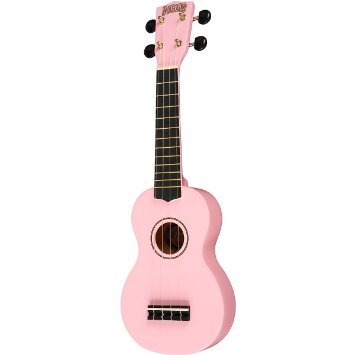
\includegraphics[width=5cm]{../img/ukulele.jpg}
\end{Slide}

\begin{Slide}{Ett stort TACK för...}
\begin{itemize}
\item ... att ni kämpat så hårt!
\item ... att ni ställt massor med frågor!
\item ... att det har varit så hög närvaro på föreläsningarna!
\item ... att ni är så konstruktiva och verkligen vill lära er!
\end{itemize}
\vspace{2em} \pause

\Alert{Ett stort LYCKA TILL på vägen till att bli en \\ kompetent och innovativ systemutvecklare!}
\end{Slide}



\fi
